
%!TEX TS-program = xelatex
\documentclass[]{friggeri-cv}
\usepackage{afterpage}
\usepackage{hyperref}
\usepackage{color}
\usepackage{xcolor}
\usepackage{smartdiagram}
\usepackage{fontspec}
% if you want to add fontawesome package
% you need to compile the tex file with LuaLaTeX
% References:
%   http://texdoc.net/texmf-dist/doc/latex/fontawesome/fontawesome.pdf
%   https://www.ctan.org/tex-archive/fonts/fontawesome?lang=en
%\usepackage{fontawesome}
\usepackage{metalogo}
\usepackage{dtklogos}
\usepackage[utf8]{inputenc}
\usepackage{tikz}
\usepackage{multicol}
\usepackage{setspace}
\usepackage[document]{ragged2e}
%\usepackage{titlesec}
%\usepackage[skip=4pt, indent=0.0pt, parfill=4.0pt]{parskip}
\usetikzlibrary{mindmap,shadows}
\hypersetup{
    pdftitle={},
    pdfauthor={},
    pdfsubject={},
    pdfkeywords={},
    colorlinks=false,           % no lik border color
    allbordercolors=white       % white border color for all
}
\smartdiagramset{
    bubble center node font = \footnotesize,
    bubble node font = \footnotesize,
    % specifies the minimum size of the bubble center node
    bubble center node size = 0.5cm,
    %  specifies the minimum size of the bubbles
    bubble node size = 0.5cm,
    % specifies which is the distance among the bubble center node and the other bubbles
    distance center/other bubbles = 0.3cm,
    % sets the distance from the text to the border of the bubble center node
    distance text center bubble = 0.5cm,
    % set center bubble color
    bubble center node color = pblue,
    % define the list of colors usable in the diagram
    set color list = {lightgray, materialcyan, orange, green, materialorange, materialteal, materialamber, materialindigo, materialgreen, materiallime},
    % sets the opacity at which the bubbles are shown
    bubble fill opacity = 0.6,
    % sets the opacity at which the bubble text is shown
    bubble text opacity = 0.5,
}

\addbibresource{bibliography.bib}
\RequirePackage{xcolor}
\definecolor{pblue}{HTML}{0395DE}

%\titlespacing*{\section}
%{0pt}{12pt plus 4pt minus 2pt}{0pt plus 2pt minus 2pt}
%\titlespacing*{\subsection}
%{0pt}{12pt plus 4pt minus 2pt}{0pt plus 2pt minus 2pt}
%\titlespacing*{\subsubsection}
%{0pt}{12pt plus 4pt minus 2pt}{0pt plus 2pt minus 2pt}
\begin{document}

\header{Yoann}{Chamillard}
      {~~~~~~~~~~~~~~~~Ingénieur Développeur Web \& Mobile Full Stack}
      {}

\begin{aside}
\hspace{10mm}
\includegraphics[scale=0.148]{res/img/Photo_CV.png}\section{Infos}
%30 ans
Permis A,B\vspace{2.5mm}
2 rue Paulin Méry
75013 Paris,
France\vspace{1.5mm}
Prêt à déménager
Mobile à l'international\vspace{2.5mm}
+33 670525552
\href{mailto:yoann.chamillard@gmail.com}{\small yoann.chamillard@gmail.com}\vspace{2.5mm}
\href{http://fr.linkedin.com/in/yoannchamillard}{LinkedIn\hspace{1.5mm}
\includegraphics[scale=0.075]{res/img/hlink.png}}
\href{https://github.com/Nokheenig?tab=stars}{GitHub\hspace{1.5mm}
\includegraphics[scale=0.075]{res/img/hlink.png}}\vspace{2.5mm}
\makebox[4.3cm][l]{\textbf{Français} }
\makebox[4.3cm][l]{\textbf{Anglais} (C1,Bulats)}
\makebox[4.3cm][l]{\textbf{Allemand} (B1)}\vspace{2.5mm}
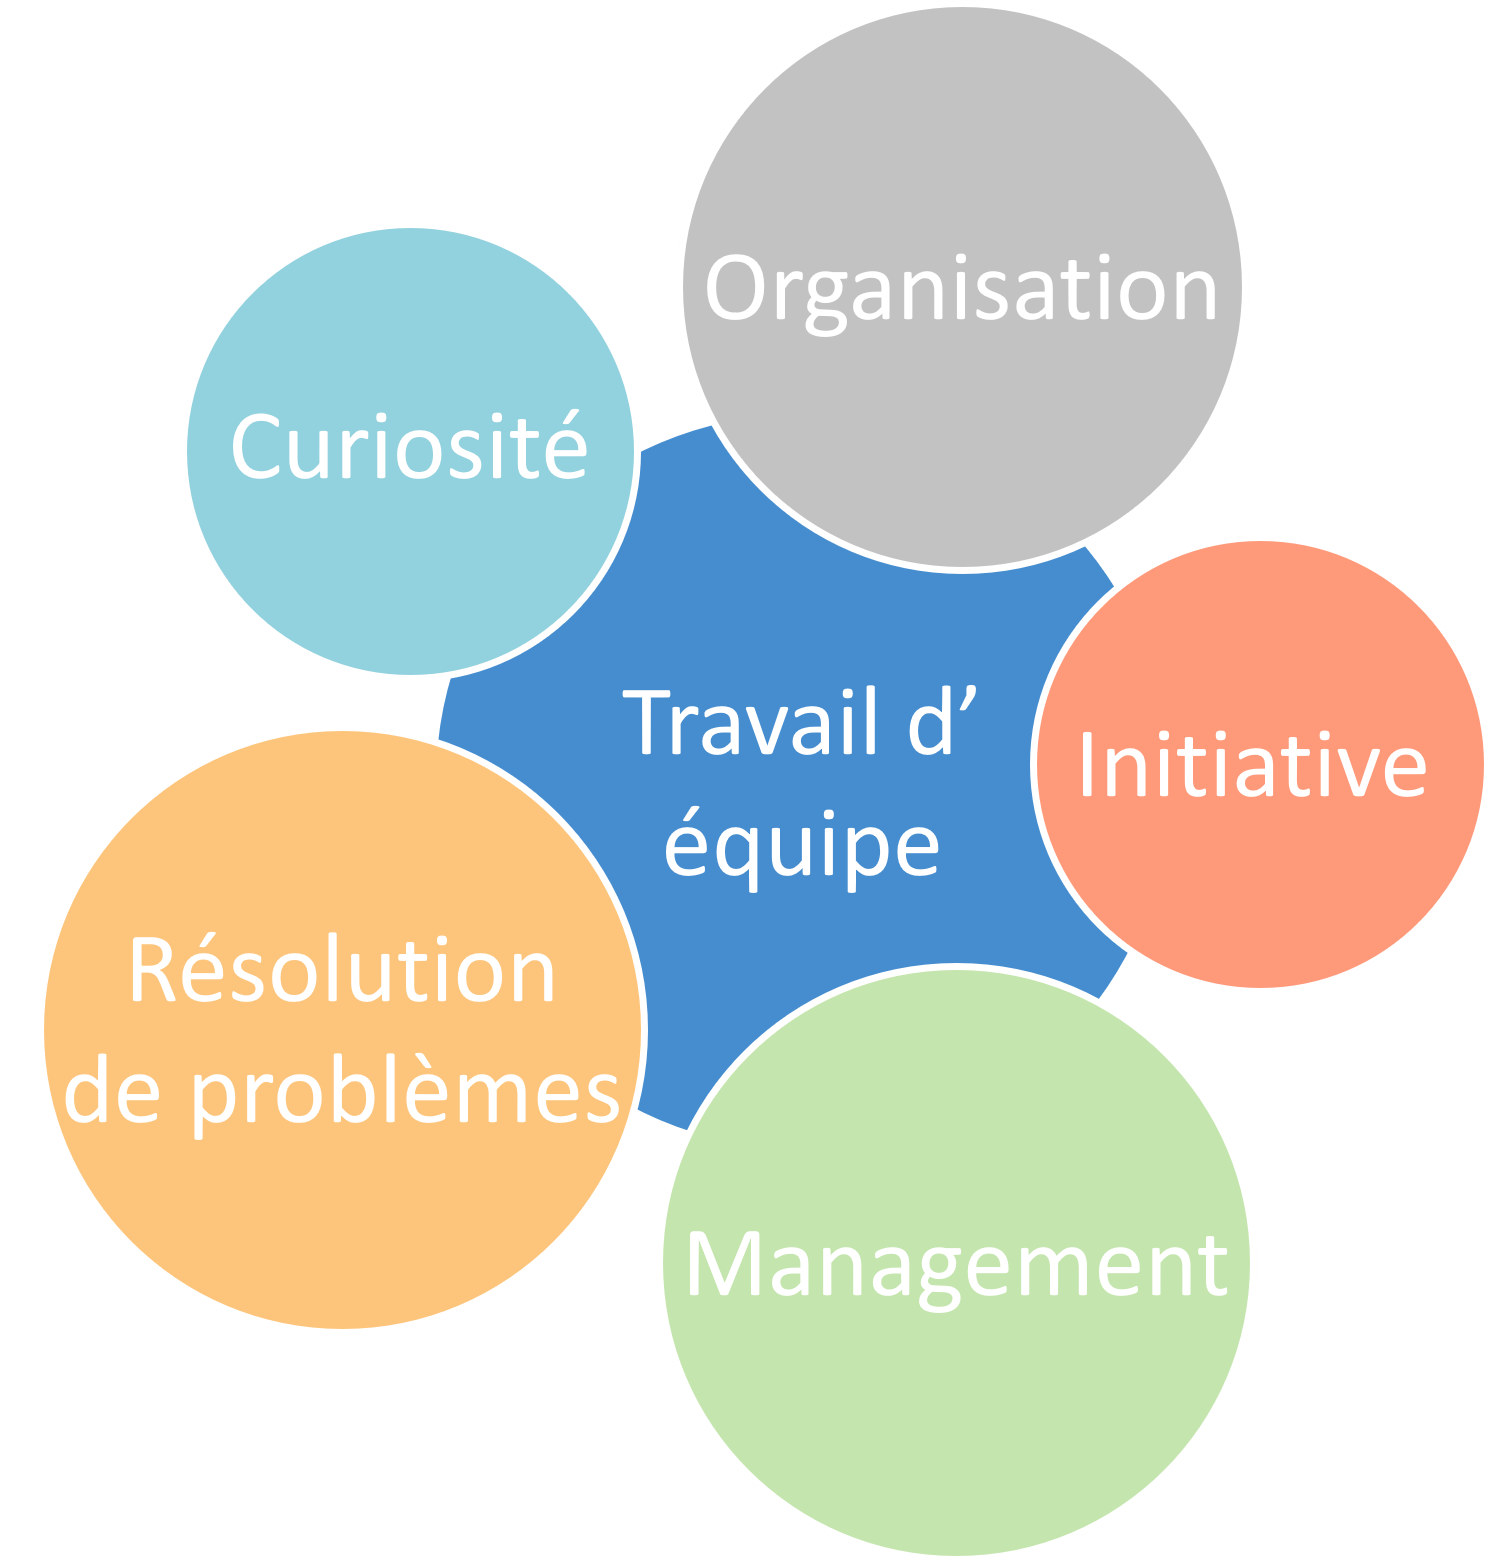
\includegraphics[scale=0.40]{res/img/profileMap_FR.png}\vspace{2.5mm}
\section{CAO / FAO}

\includegraphics[scale=0.40]{res/img/5stars.png}\hspace{1.5mm}\textbf{Catia V5\&V6}

\includegraphics[scale=0.40]{res/img/4stars.png}\hspace{1.5mm}\textbf{Creo 4.0}

\includegraphics[scale=0.40]{res/img/3stars.png}\hspace{1.5mm}\textbf{Impression 3D}\section{PLM / PDM}

\includegraphics[scale=0.40]{res/img/4stars.png}\hspace{1.5mm}\textbf{NewPDM}

\includegraphics[scale=0.40]{res/img/3stars.png}\hspace{1.5mm}\textbf{Windchill}\section{Calcul / FEM}

\includegraphics[scale=0.40]{res/img/3stars.png}\hspace{1.5mm}\textbf{Ansys Wbench}

\includegraphics[scale=0.40]{res/img/3stars.png}\hspace{1.5mm}\textbf{Abaqus}

\includegraphics[scale=0.40]{res/img/2-5stars.png}\hspace{1.5mm}\textbf{Hyperworks}

\includegraphics[scale=0.40]{res/img/2-5stars.png}\hspace{1.5mm}\textbf{Hypermesh}
\vspace{2.5mm}%\begin{flushleft}
	\emph{Le 12/6/2024} \hspace*{8mm}
	%\end{flushleft}
\end{aside}
\section{Compétences informatiques}
        \vspace*{-0.45cm}
        \setlength{\columnsep}{-0.3cm}
        \begin{flushleft}
        \begin{multicols}{3}
		\begin{itemize}
		
		\setlength{\itemsep}{5pt}
  		\setlength{\parskip}{0pt}
  		\setlength{\parsep}{0pt}
          
        
\item \large Mobile \
\normalsize
\begin{flushleft}


\includegraphics[scale=0.40]{res/img/4stars.png}\hspace{1.5mm}\textbf{Kotlin}\\Room, Firebase, Gson, Jetpack Compose, Retrofit, MVVM, Coroutine\\\vspace{2mm}

\includegraphics[scale=0.40]{res/img/4stars.png}\hspace{1.5mm}\textbf{Flutter}

\includegraphics[scale=0.40]{res/img/4stars.png}\hspace{1.5mm}\textbf{Android}
\end{flushleft}            

\item \large Developpement web \
\normalsize
\begin{flushleft}


\includegraphics[scale=0.40]{res/img/4stars.png}\hspace{1.5mm}\textbf{HTML,CSS}

\includegraphics[scale=0.40]{res/img/4stars.png}\hspace{1.5mm}\textbf{JavaScript}
\end{flushleft}            

\item \large Frameworks web \
\normalsize
\begin{flushleft}


\includegraphics[scale=0.40]{res/img/4stars.png}\hspace{1.5mm}\textbf{Django}

\includegraphics[scale=0.40]{res/img/4stars.png}\hspace{1.5mm}\textbf{Vue.Js}

\includegraphics[scale=0.40]{res/img/3stars.png}\hspace{1.5mm}\textbf{PHP-Laravel}
\end{flushleft}            

\columnbreak
\item \large Application / Serveur \
\normalsize
\begin{flushleft}


\includegraphics[scale=0.40]{res/img/5stars.png}\hspace{1.5mm}\textbf{Python}\\Flask, SQLAlchemy, PyMongo, PyTest, FastAPI, Numpy\\\vspace{2mm}

\includegraphics[scale=0.40]{res/img/3stars.png}\hspace{1.5mm}\textbf{Java}

\includegraphics[scale=0.40]{res/img/3stars.png}\hspace{1.5mm}\textbf{Nginx}

\includegraphics[scale=0.40]{res/img/3stars.png}\hspace{1.5mm}\textbf{Apache}

\includegraphics[scale=0.40]{res/img/4stars.png}\hspace{1.5mm}\textbf{API}
\end{flushleft}            

\item \large Authentification \
\normalsize
\begin{flushleft}


\includegraphics[scale=0.40]{res/img/4stars.png}\hspace{1.5mm}\textbf{JWT Auth}

\includegraphics[scale=0.40]{res/img/3stars.png}\hspace{1.5mm}\textbf{OAuth}

\includegraphics[scale=0.40]{res/img/4stars.png}\hspace{1.5mm}\textbf{Firebase}
\end{flushleft}            

\item \large Devops, CI/CD \
\normalsize
\begin{flushleft}


\includegraphics[scale=0.40]{res/img/4stars.png}\hspace{1.5mm}\textbf{Git / GitLab}

\includegraphics[scale=0.40]{res/img/3stars.png}\hspace{1.5mm}\textbf{Docker}

\includegraphics[scale=0.40]{res/img/3stars.png}\hspace{1.5mm}\textbf{Jenkins}

\includegraphics[scale=0.40]{res/img/3stars.png}\hspace{1.5mm}\textbf{Selenium}

\includegraphics[scale=0.40]{res/img/3stars.png}\hspace{1.5mm}\textbf{Cron}
\end{flushleft}            

\columnbreak
\item \large Bases de données \
\normalsize
\begin{flushleft}


\includegraphics[scale=0.40]{res/img/4stars.png}\hspace{1.5mm}\textbf{MySQL}

\includegraphics[scale=0.40]{res/img/3stars.png}\hspace{1.5mm}\textbf{PostgreSQL}

\includegraphics[scale=0.40]{res/img/4stars.png}\hspace{1.5mm}\textbf{MongoDB}

\includegraphics[scale=0.40]{res/img/3stars.png}\hspace{1.5mm}\textbf{SQLite}
\end{flushleft}            

\item \large Data \
\normalsize
\begin{flushleft}


\includegraphics[scale=0.40]{res/img/4stars.png}\hspace{1.5mm}\textbf{Shiny}

\includegraphics[scale=0.40]{res/img/4stars.png}\hspace{1.5mm}\textbf{Pandas}

\includegraphics[scale=0.40]{res/img/4stars.png}\hspace{1.5mm}\textbf{Matplotlib}

\includegraphics[scale=0.40]{res/img/4stars.png}\hspace{1.5mm}\textbf{Jupyter}
\end{flushleft}            

\item \large IA \& Outils \
\normalsize
\begin{flushleft}


\includegraphics[scale=0.40]{res/img/3stars.png}\hspace{1.5mm}\textbf{Tensorflow}

\includegraphics[scale=0.40]{res/img/3stars.png}\hspace{1.5mm}\textbf{Keras}
\end{flushleft}            

\item \large Autres \
\normalsize
\begin{flushleft}


\includegraphics[scale=0.40]{res/img/3stars.png}\hspace{1.5mm}\textbf{Bash}

\includegraphics[scale=0.40]{res/img/4stars.png}\hspace{1.5mm}\textbf{OpenAPI}

\includegraphics[scale=0.40]{res/img/4stars.png}\hspace{1.5mm}\textbf{Jira}
\end{flushleft}            


        \end{itemize}
        \end{multicols}
        %\end{itemize}
        \end{flushleft} \normalsize
        \vspace*{-0.65cm}
\section{Expériences}
\vspace*{-0.25cm}

\begin{entrylist}
  \entry
    {09/22 - 11/23}
    {Développeur web \& mobile}
    {Synapsun, \textit{Lyon, FR}}
    {Développements fullstack web \& mobile Android:\hspace*{8mm}Flutter, Python, Kotlin}
\end{entrylist}
\vspace{-10pt}
\begin{minipage}[t]{0.65\linewidth}
\underline{Contexte - Mission: }\\
Automatiser et améliorer la réactivité du service de repowering (identifier et proposer des panneaux solaires de remplacement aux exploitants de centrales solaire endommagées ou vieillissantes)\\
\end{minipage} % no space if you would like to put them side by side
\begin{minipage}[t]{0.38\textwidth}
    \underline{Envir. Technique: }\
    \vspace{1mm}
    
\underline{\textit{Mobile}}: Android, Flutter, Kotlin\\
\underline{\textit{Web}}: Python, Django, Javascript, PHP, HTML, CSS\\
\underline{\textit{Devops, CI/CD}}: Git, GitLab\\
\underline{\textit{Bases de données}}: PostgreSQL, MongoDB\\
\underline{\textit{Langues}}: Français, Anglais (équipe internationale)\\
\underline{\textit{Autres}}: OpenAPI, API, Jira, VBA
    \end{minipage}
\vspace{1.5mm}
\underline{Finalité: }\\

\begin{itemize}
\setlength{\itemsep}{1pt}
\setlength{\parskip}{0pt}
\setlength{\parsep}{0pt}

\item Soulager le service commercial dans le traitement des dossiers de repowering et améliorer le temps de réponse au client
\item Identifier et accéder instantanément aux caractéristiques des panneaux de l'installation du client
\item Automatiser la recherche de panneaux compatibles au catalogue de la société ou disponibles chez nos fournisseurs
\item Fournir aux clients une appli mobile pour le guider jusqu'à l'émission d'une demande de devis sur les références compatibles identifiées.
\end{itemize}

\vspace{1.5mm}
\underline{Tâches - Réalisations: }\\

\begin{itemize}
\setlength{\itemsep}{1pt}
\setlength{\parskip}{0pt}
\setlength{\parsep}{0pt}

\item Recueil du besoin, construction d'un cahier des charges et de spécifications fonctionnelles et techniques.
\item Développement d'un web scraper en Python
\item Conception de modèles de données
\item Rédaction de spécifications d'API au standard OpenAPI / Swagger
\item Mise en place d'une base de données produits MongoDB et d'une API Python FastAPI
\item Développement d'un client mobile multi-plateforme Flutter.
\item Gestion des accès par token JWT (Json Web Token)
\item Mise en place d'une base de données PostgreSQL et d'un back-end Python Django pour la gestion des utilisateurs et des devis.
\item Contact fournisseur/prestataire pour les travaux outsourcés
\end{itemize}

\begin{entrylist}
  \entry
    {11/19 - 04/22}
    {Ingénieur développement produit}
    {Böllhoff (via Davricourt), \textit{Chambéry, FR}}
    {Conception produit mécatronique automobile}
\end{entrylist}
\vspace{-10pt}
\begin{minipage}[t]{0.65\linewidth}
\underline{Contexte - Mission: }\\
Service R\&D Innovation, développement d'une nouvelle gamme de produits à haute valeur ajoutée - fixations et Systèmes d'assemblage instrumentés.\\
\end{minipage} % no space if you would like to put them side by side
\begin{minipage}[t]{0.38\textwidth}
    \underline{Envir. Technique: }\
    \vspace{1mm}
    
\underline{\textit{CAD}}: DS Catia V5, PTC Creo 7\\
\underline{\textit{PDM}}: Windchill\\
\underline{\textit{CAE}}: Ansys Workbench, Creo Simulate, Altair Simsolid\\
\underline{\textit{DOE, Statistiques}}: Minitab\\
\underline{\textit{Extensométrie, Acquisition}}: Jauges de déformation pelliculaires HBM, Catman Easy, Multimètre Oscilloscope Kickstart\\
\underline{\textit{Langues}}: Français, Anglais (équipe internationale)\\
\underline{\textit{Autres}}: Excel, Powerpoint, VBA
    \end{minipage}
\vspace{1.5mm}
\underline{Tâches - Réalisations: }\\

\begin{itemize}
\setlength{\itemsep}{1pt}
\setlength{\parskip}{0pt}
\setlength{\parsep}{0pt}

\item Définition produit et produits liés au(x) process/essais (Géométrie, Simu/Calcul, Dimensionnement, Optimisation, Interfaces): Capteurs, Assemblages vissés sous précontrainte, Élément fixé sur caisse (réservoir, coffre de toit, ...), Élément de suspension/train (McPherson, Torsible, à lames), Machine spéciale (collage, préhension/commande pneumatique)
\item Mise en plan, Cotation fonctionnelle, Chaines de cotes (Arithmétiques, Quadratiques)
\item Assurer les jeux avec l'environnement (Archi, Thermiques,...)
\item Assurer la montabilité, la mise et maintien en position des produits par les moyens de montage
\item Rédaction de méthodes d’essai et réalisation d’essais de validation : Essais Labo, Sous-Système et Système, Essais de flexion, Essais de traction-compression
\item Plans d’Expérience/Taguchi/Design-Of-Experiments : Définition, Analyse
\item Extensométrie, Acquisition: Vérifier la tenue mécanique et la concordance des prototypes avec leur modèle simu à l’aide de jauges de déformation pelliculaires (HBM)
\item Plasturgie : Conception de pièces de boitier module avec fonctions d’étanchéité
\item Prototypage 3D FDM, Consultation fournisseur
\item Participation aux design review : présentation synthétique des problèmes, établissement de plans d’action, suivi de leur application
\end{itemize}

\begin{entrylist}
  \entry
    {11/16 - 09/19}
    {Ingénieur d'étude automobile}
    {Renault (via Bertrandt), \textit{Vélizy, FR}}
    {Conception \& architecture sous-caisse et compartiment moteur}
\end{entrylist}
\vspace{-10pt}
\begin{minipage}[t]{0.65\linewidth}
\underline{Contexte - Mission: }\\
Service Architecture/Powertrain - Conception d'équipements véhicule:\\11/16>03/17: Renault Zoé Ph.2 (Véhicule électrique) Conception/archi compartiment moteur/Sous-caisse;\\ 08/17>07/19: PHEV (Hybride Rechargeable), Plateformes CMF1/CMF-B, Conception et pilotage conception-archi Sous-caisse;\\04/19>09/19: Euro7 \& HEV (Hybride), Plateforme Utilitaire CD1, Conception et pilotage Sous-caisse.\\
\end{minipage} % no space if you would like to put them side by side
\begin{minipage}[t]{0.38\textwidth}
    \underline{Envir. Technique: }\
    \vspace{1mm}
    
\underline{\textit{CAD}}: DS Catia V6\\
\underline{\textit{PDM}}: NewPDM\\
\underline{\textit{Langues}}: Français, Anglais (équipe internationale)\\
\underline{\textit{Autres}}: Excel, Powerpoint, VBA
\vspace{25mm}
    \end{minipage}
\vspace{1.5mm}
\underline{Tâches - Réalisations: }\\

\begin{itemize}
\setlength{\itemsep}{1pt}
\setlength{\parskip}{0pt}
\setlength{\parsep}{0pt}

\item Définition produit (Géométrie, Interfaces): Tout type de pièce dans les zones d'architecture concernées.
\item Assurer les jeux avec l'environnement (Archi, Thermiques,...) avec les pièces fixes et mobiles
\item Assurer la montabilité, la mise et maintien en position des produits par les moyens de montage autos et manuels
\item Mise en plan, Cotation fonctionnelle, Chaines de cotes (Arithmétiques, Quadratiques)
\item Suivi de convergence du périmètre archi
\item Animation de groupe de travail (Pilotage de concepteurs français et à l'étranger)
\item Organisation et animation de design review : présentation synthétique des problèmes, établissement de plans d’action, suivi de leur application
\end{itemize}

\vspace*{-0.5cm}
\vspace*{0.45cm}
\section{Formations - Certifications}
\vspace*{-0.25cm}
\vspace{0.5mm}
\begin{entrylist}
  \entry
    {09/22 - 08/23}
    {Bachelor Concepteur Développeur d'Applications}
    {EPSI, \textit{Lyon, FR}}
    {RNCP Niv.6 - Spécialité Data/IA; \hspace{7mm} 09/23: Certification d'état CDA}
\end{entrylist}
\vspace*{-0.65cm}
\begin{itemize}
\setlength{\itemsep}{1pt}
\setlength{\parskip}{0pt}
\setlength{\parsep}{0pt}
\begin{multicols}{2}
\item Développement: \newline Java, Python, Dart/Flutter, etc.
\columnbreak
\item Data, Bases de données, etc.
\item Tests et intégration continue (CI/CD)
\end{multicols}
\end{itemize}\vspace{0.5mm}
\begin{entrylist}
  \entry
    {06/22 - 08/22}
    {Formation d'Intégrateur-développeur web}
    {Epitech, \textit{Paris, FR}}
    {RNCP Niv.5}
\end{entrylist}

\vspace*{-0.35cm}
\begin{itemize}
\setlength{\itemsep}{1pt}
\setlength{\parskip}{0pt}
\setlength{\parsep}{0pt}

\item PHP, HTML, CSS, JavaScript, Vue.Js, Laravel, Bash, Git
\end{itemize}\vspace{0.5mm}
\begin{entrylist}
  \entry
    {09/13 - 08/16}
    {Diplôme d'Ingénieur en Systèmes Mécaniques}
    {UTT, \textit{Troyes, FR}}
    {RNCP Niv.7; Conception et Industrialisation, en lien avec l’Environnement}
\end{entrylist}
\vspace{0.5mm}
\begin{entrylist}
  \entry
    {09/11 - 06/13}
    {DUT Génie Mécanique et Productique}
    {IUT, \textit{Troyes, FR}}
    {RNCP Niv.5}
\end{entrylist}
\vspace*{-0.4cm}
\begin{itemize}
\setlength{\itemsep}{1pt}
\setlength{\parskip}{0pt}
\setlength{\parsep}{0pt}
\item Conception, dimensionnement, asservissement et programmation d’un robot pour participer à la coupe de France de robotique (E=M6)
\end{itemize}
\section{Centres d'intérêt}
\vspace*{-0.45cm}
\setlength{\columnsep}{-2cm}
\begin{multicols}{2}
\begin{itemize}
\setlength{\itemsep}{1pt}
\setlength{\parskip}{0pt}
\setlength{\parsep}{0pt}
\item Sorties: \\
Randonnée, Concerts,  Moto, Photo\\
\item Musique: \\
Batterie, Piano\\
\columnbreak
\item Voyages: \\
Suède, Cambodge, Thaïlande, Allemagne\\
\item Lecture: \\
B.Werber, M.Chattam, F.Thilliez
\end{itemize}
\end{multicols}
\end{document}